\documentclass[english,9pt,aspectraio=169]{beamer}
\usepackage{etex}
\usetheme{uzhneu-en-informal}
%\usepackage{uarial}
\usepackage[T1]{fontenc}
\usepackage[utf8]{inputenc}
\RequirePackage{graphicx,ae}
\usepackage{bm}
\usepackage{fancybox,amssymb,color}
\usepackage{pgfpages}
\usepackage{booktabs}
\usepackage{verbatim}
\usepackage{animate}
\usepackage{numprint}
\usepackage{dsfont}
\usepackage{tikz}
\usepackage{amsmath,natbib}
\usepackage{mathbbol}
\usepackage{babel}
\usepackage{SweaveSlides}
\usepackage{multicol}
\usepackage{xcolor}


\usetheme{uzhneu-en-informal}
\DeclareMathOperator{\po}{Poisson}
\DeclareMathOperator{\G}{Gamma}
\DeclareMathOperator{\Be}{Beta}
\DeclareMathOperator{\logit}{logit}
\def\n{\mathop{\mathcal N}}

\definecolor{Gray}{RGB}{139,137,137}
\definecolor{darkred}{rgb}{0.8,0,0}
\definecolor{Green}{rgb}{0,0.8,0.3}
\definecolor{Blue}{rgb}{0,0,1}
\def\myalert{\textcolor{darkred}}
\def\myref{\textcolor{Gray}}
\setbeamercovered{invisible}

\renewcommand{\baselinestretch}{1.2}
\beamertemplateballitem
\DeclareMathOperator{\cn}{cn} % Copy number
\DeclareMathOperator{\ccn}{ccn} % common copy number
\DeclareMathOperator{\p}{p} % common copy number
\DeclareMathOperator{\E}{E} % common copy number
\DeclareMathOperator{\given}{|} % common copy number
\def\given{\,|\,}
\def\na{\tt{NA}}
\def\nin{\noindent}
\pdfpageattr{/Group <</S /Transparency /I true /CS /DeviceRGB>>}
\def\eps{\varepsilon}

\renewcommand{\P}{\operatorname{\mathsf{Pr}}} % Wahrscheinlichkeitsmaß
\def\eps{\varepsilon}
\def\logit{\text{logit}}
%\newcommand{\E}{\mathsf{E}} % Erwartungswert
\newcommand{\Var}{\text{Var}} % Varianz
\newcommand{\NBin}{\text{NBin}}
\newcommand{\Po}{\text{Po}}
\newcommand{\N}{\mathsf{N}}

\newcommand{\ball}[1]{\begin{pgfpicture}{-1ex}{-0.65ex}{1ex}{1ex}
\usebeamercolor[fg]{item projected}

{\pgftransformscale{1.75}\pgftext{\normalsize\pgfuseshading{bigsphere}}}
{\pgftransformshift{\pgfpoint{0pt}{0.5pt}}
\pgftext{\usebeamerfont*{item projected}{#1}}}
\end{pgfpicture}}%
\usepackage{multicol}
\newcommand{\ballsmall}[1]{\begin{pgfpicture}{-1ex}{-0.65ex}{.2ex}{.2ex}

{\pgftransformscale{1}\pgftext{\normalsize\pgfuseshading{bigsphere}}}
{\pgftransformshift{\pgfpoint{0pt}{0.5pt}}
\pgftext{\usebeamerfont*{item projected}{#1}}}
\end{pgfpicture}}%




\begin{document}
\begin{Schunk}
\begin{Sinput}
> library(reporttools)
> library(biostatUZH)
\end{Sinput}
\end{Schunk}

\fboxsep5pt

\frame{
\title[]{ \centering \Huge Kurs Bio144: \\
Datenanalyse in der Biologie}%\\[.3cm]
\author[Stefanie Muff, Owen L.\ Petchey]{\centering Stefanie Muff  \& Owen L.\ Petchey }
%\institute[]{Institute of Social and Preventive Medicine \\ Institute of Evolutionary Biology and Environmental Studies}
\date[]{Week 3: Multiple linear regression \\ 9./10. March 2017}


\maketitle
}


\frame{\frametitle{Overview (todo: check)}
\begin{itemize}
\item Multiple predictors $x_1$, $x_2$, \ldots, $x_p$
\item $R^2$ in multiple linear regression
\item $t$-tests, $F$-tests and $p$-values
\item Binary and factor covariates
\item Interactions between covariates
\item Multiple vs.\ many single regressions
\end{itemize}
}



\frame{\frametitle{Course material covered today}
\begin{itemize}
\item Chapters 3.1 - 3.3 of \emph{Lineare Regression}, p.25-39 (Stahel script)
\item Other?
\end{itemize}
}

\frame[containsverbatim]{\frametitle{Recap of last week I}

\begin{itemize}
\item The linear regression model for the data $\bm{y}=(y_1,\ldots,y_n)$ given $\bm{x}=(x_1,\ldots,x_n)$ is
$$y_i = \alpha + \beta x_i + E_i \ , \qquad E_i \sim \N(0,\sigma_E^2) \  \text{independent}.$$\\[2mm]
\item Estimate the parameters $\alpha$, $\beta$ and $\sigma_E^2$ by least squares.\\[2mm]
\item The estimated parameters $\hat\alpha$, $\hat\beta$ contain \myalert{uncertainty} and are normally distributed around the true values. %(actually, also $\hat\sigma_E^2$...). \\[2mm]
\item Knowing this helps to deduce \myalert{statistical tests}, such as: Is $\beta=0$?\\[2mm]
\item Testing is simple using R:\\[2mm]
\begin{Schunk}
\begin{Sinput}
> summary(r.bodyfat)$coef
\end{Sinput}
\begin{Soutput}
              Estimate Std. Error   t value     Pr(>|t|)
(Intercept) -26.984368  2.7689004 -9.745518 3.921511e-19
bmi           1.818778  0.1083411 16.787522 2.063854e-42
\end{Soutput}
\end{Schunk}
\end{itemize}

}


\frame[containsverbatim]{\frametitle{Recap of last week II}

\begin{itemize}
\item Confidence and prediction ranges:
\end{itemize}
\begin{center}
\setkeys{Gin}{width=0.65\textwidth}
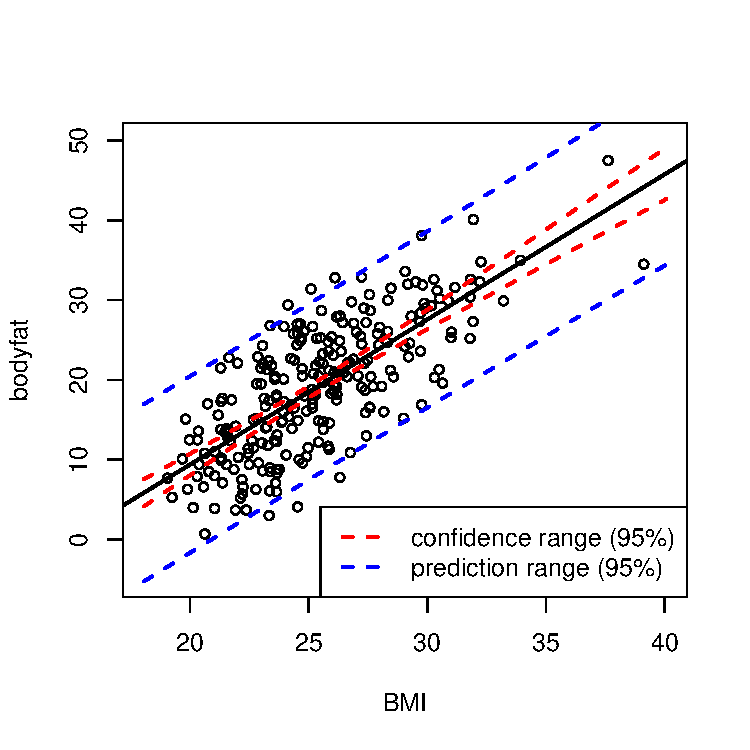
\includegraphics{Bio144_2017_week3-confpred}
\end{center}
}


\frame[containsverbatim]{\frametitle{Bodyfat example}
We have so far modelled bodyfat in dependence of bmi, that is: $(body fat)_i = \alpha + \beta \cdot bmi_i + E_i$.\\[2mm]

However, other predictors might also be relevant for an accurate prediction of bodyfat.\\[4mm]

{\bf Examples:} Age, neck fat (Nackenfalte), hip circumference, abdomen circumference etc.
\begin{center}
\setkeys{Gin}{width=1\textwidth}
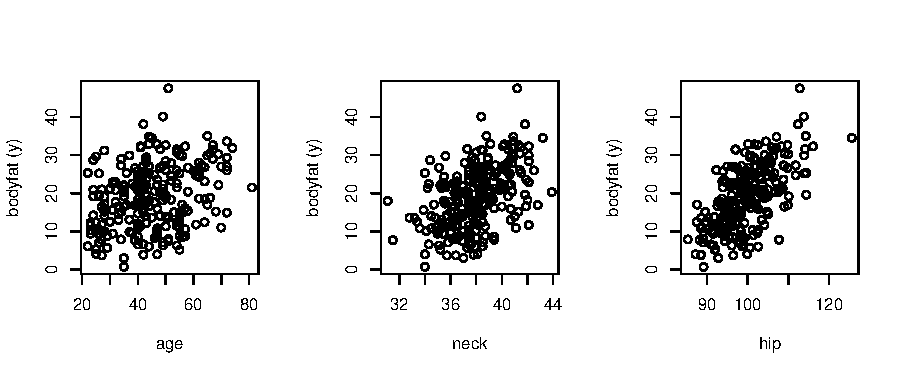
\includegraphics{Bio144_2017_week3-005}
\end{center}

}


\frame[containsverbatim]{\frametitle{Multiple linear regression model}
The idea is simple: just {\bf extend the linear model by additional predictors}.\\[4mm]

\begin{itemize}
\item Given several influence factors $x_i^{(1)}$, \ldots, $x_i^{(m)}$, 
the straightforward extension of the simple linear model is\\[4mm]

\colorbox{lightgray}{\begin{minipage}{10cm}
\begin{eqnarray*}
y_i &=& \beta_0 + \beta_1 x_i^{(1)} + \beta_2 x_i^{(2)} + \ldots + \beta_2 x_i^{(m)} + E_i  \\[2mm]
\text{with  } \ E_i &\sim& \N (0,\sigma_E^2).
\end{eqnarray*}
\end{minipage}}
~\\[6mm]
\item The parameters of this model are $\bm\beta=(\beta_0,\beta_1,\ldots,\beta_m)$ and $\sigma_E^2$.
\end{itemize}
}

\frame{\frametitle{}
The components of $\bm\beta$ are again estimated using the {\bf least squares} method. Basically, the idea is (again) to minimize 
$$\sum_{i=1}^n r_i^2$$
with 
$$r_i = y_i - (\beta_0 + \beta_1 x_i^{(1)} + \beta_2 x_i^{(2)} + \ldots + \beta_2 x_i^{(m)}) $$ 

It is a bit more complicated than for simple linear regression, see Sections 3.3 and 3.4 of the Stahel script. \\[4mm]

Some {\bf linear algebra} is needed to understand these sections, but we do not look into this for the moment. (It will come later in week 6.) \\[4mm]


}

\frame[containsverbatim]{\frametitle{Multiple linear regression with R}
\vspace{-5mm}
Let us fit bodyfat (from last week) to the predictors {\bf bmi} and {\bf age} simultaneously. The R code to fit the model is\\[2mm]

\begin{Schunk}
\begin{Sinput}
> r.bodyfatM <- lm(bodyfat ~ bmi + age ,d.bodyfat)#+ neck + hip + abdomen
\end{Sinput}
\end{Schunk}
\begin{Schunk}
\begin{Sinput}
> summary(r.bodyfatM)
\end{Sinput}
\begin{Soutput}
Call:
lm(formula = bodyfat ~ bmi + age, data = d.bodyfat)

Residuals:
     Min       1Q   Median       3Q      Max 
-12.0415  -3.8725  -0.1237   3.9193  12.6599 

Coefficients:
             Estimate Std. Error t value Pr(>|t|)    
(Intercept) -31.25451    2.78973 -11.203  < 2e-16 ***
bmi           1.75257    0.10449  16.773  < 2e-16 ***
age           0.13268    0.02732   4.857 2.15e-06 ***
---
Signif. codes:  0 ‘***’ 0.001 ‘**’ 0.01 ‘*’ 0.05 ‘.’ 0.1 ‘ ’ 1

Residual standard error: 5.329 on 240 degrees of freedom
Multiple R-squared:  0.5803,	Adjusted R-squared:  0.5768 
F-statistic: 165.9 on 2 and 240 DF,  p-value: < 2.2e-16
\end{Soutput}
\end{Schunk}
}

\frame[containsverbatim]{\frametitle{}
Which questions should be asked? (In principle, we should have asked the questions \emph{before}!)\\[6mm]
\begin{enumerate}
\item Does the {\bf ensemble} of all covariates influence the response?\\[4mm]
\item If yes, which influence variables are good predictors of bodyfat? \\[4mm]
\item How good is the model fit?
\end{enumerate}

}



\frame[containsverbatim]{\frametitle{Question 1: Does the model have some explanatory power?}
To answer question 1, we need to perform a so-called $F$-test. The results of the test are displayed in the final line of the regression summary. Here, it says:\\[2mm]

\texttt{F-statistic: 165.9 on 2 and 240 DF, p-value: < 2.2e-16} \\[2mm]

So apparently (and we already suspected that) the model has some explanatory power.\\[8mm]

\scriptsize{
*The $F$-statistic and -test is briefly recaptured in 3.1.f) of the Stahel script, but see also Mat183 chapter 6.2.5. It uses the fact that
%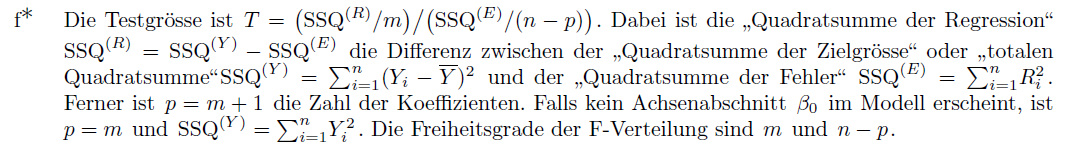
\includegraphics[width=11cm]{pictures/fstar.jpg}
\begin{equation*}
\frac{SSQ^{(R)}/m}{SSQ^{(E)}/(n-p)} \sim F_{m,n-p}
\end{equation*}
follows an $F$-distribution (\texttt{df()} in R) with $m$ and $(n-p)$ degrees of freedom, where $m$ are the number of variables, $n$ the number of data points, $p$ the number of $\beta$-parameters (typically $m+1$). $SSQ^{(E)}=\sum_{i=1}^nR_i^2$ is the squared sum of the residuals, and $SSQ^{(R)} = SSQ^{(Y)} - SSQ^{(E)}$ with $SSQ^{(y)}=\sum_{i=1}^n(y_i-\overline{y})^2$.
}

}

\frame[containsverbatim]{\frametitle{Question 2: Which variables influence the response?}
%' <<summary.bf,results=tex,echo=F>>= 
%' tableRegression(r.bodyfatM)
%' @

\begin{Schunk}
\begin{Sinput}
> summary(r.bodyfatM)$coef
\end{Sinput}
\begin{Soutput}
               Estimate Std. Error    t value     Pr(>|t|)
(Intercept) -31.2545057 2.78973238 -11.203406 1.039096e-23
bmi           1.7525705 0.10448723  16.773060 2.600646e-42
age           0.1326767 0.02731582   4.857137 2.149482e-06
\end{Soutput}
\end{Schunk}
~\\[2mm]

To answer this question, again look at the $t$-tests, for which the $p$-values are given in the final column. Each $p$-value refers to the test for the null hypothesis $ \beta^{(j)}_0=0$ for covariate $x^{(j)}$.\\[2mm]

As in simple linear regression, the $T$-statistic for the $j$-th covariate is calculated as 
%
\begin{equation}\label{eq:beta}
T_j =\frac{\hat\beta_j - {\beta_j}_0}{se^{(\beta_j)}}  \quad\underbrace{=}_{if  {\beta_j}_0=0} \quad  \frac{\hat\beta_j}{se^{(\beta_j)}}\ ,
\end{equation}
with  $se^{(\beta_j)}$ given in the second column of the regression output.\\[2mm]


}

\frame{

Therefore:  A ``small'' $p$-value indicates that the variable is relevant in the model.\\[2mm]

Here, we have 
\begin{itemize}
\item $p<0.001$ for bmi
\item $p<0.001$ for age
\end{itemize}

Thus both, bmi and age seem to have some predictive power for bodyfat. \\[6mm]

{\bf !However!: } \\[2mm]
The $p$-value and $T$-statistics should only be used as a {\bf rough guide} for the ``significance'' of the coefficients. 


}


\frame[containsverbatim]{\frametitle{ }

For illustration, let us extend the model a bit more:\\[4mm]

\begin{Schunk}
\begin{Sinput}
> r.bodyfatM2 <- lm(bodyfat ~ bmi + age + neck + hip + abdomen,d.bodyfat)
> summary(r.bodyfatM2)$coef
\end{Sinput}
\begin{Soutput}
               Estimate Std. Error    t value     Pr(>|t|)
(Intercept) -7.74964673 7.29830233 -1.0618424 2.893881e-01
bmi          0.42647368 0.23132902  1.8435805 6.649276e-02
age          0.01457356 0.02782994  0.5236649 6.010010e-01
neck        -0.80206081 0.19096606 -4.2000177 3.779800e-05
hip         -0.31764315 0.10751209 -2.9544876 3.447492e-03
abdomen      0.83909391 0.08417902  9.9679702 9.035870e-20
\end{Soutput}
\end{Schunk}
~\\[3mm]
It is now much \myalert{less clear what the influences of age ($p=0.60$) and bmi ($p=0.06$) are}. \\[2mm]

Basically, the problem is that the variables in the model are already correlated and therefore explain similar aspects that influence the proportion of bodyfat. \\[2mm]

This problem is at the heart of many confusions of regression analysis, and we will talk about such issues later in the course.\\[2mm]




}

\frame[containsverbatim]{\frametitle{Question 3: How good is the overall model fit?}
To answer this question, we can look at the \myalert{multiple $R^2$} (see Stahel 3.1.h). It is a generalized version of $R^2$ for simple linear regression:\\[2mm]

\colorbox{lightgray}{\begin{minipage}{10cm}
$R^2$ {\bf for multiple linear regression} is defined as the squared correlation between $(y_1,\ldots,y_n)$ and $(\hat{y}_1,\ldots,\hat{y}_n)$, where the $\hat y$ are the fitted values 
\begin{equation*}
\hat{y}_i = \hat\beta_0 + \hat\beta_1 x^{(1)} + \ldots + \hat\beta_m x^{(m)}
\end{equation*}
\end{minipage}}
\vspace{-5mm}
\begin{center}
\setkeys{Gin}{width=0.5\textwidth}
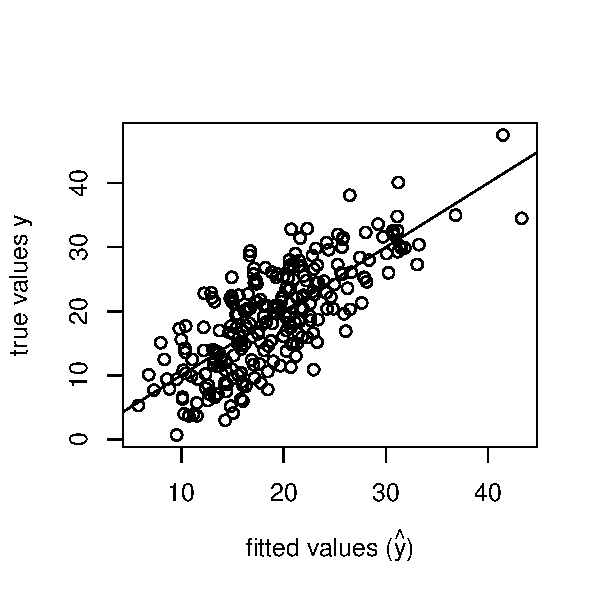
\includegraphics{Bio144_2017_week3-011}
\end{center}
}


\frame{
$R^2$ is also called the \emph{coefficient of determination} or \myalert{``Bestimmtheitsmass''}, because it measures the proportion of the reponse's variability that is explained by the ensemble of all covariates:\\[4mm]

\colorbox{lightgray}{\begin{minipage}{10cm}
\begin{equation*}
R^2 = SSQ^{(R)} / SSQ^{(Y)} = 1 - SSQ^{(E)}/ SSQ^{(Y)}
\end{equation*}
\end{minipage}}
~~\\
Remembering that \\
\begin{eqnarray*}
\text{total variability} &=&  \text{explained variability} + \text{residual variability} \\[2mm]
\sum_{i=1}^n (y_i - \overline{y})^2 &=&  \sum_{i=1}^n (\hat{y_i}-\overline{y})^2 \qquad \quad + \quad \qquad \sum_{i=1}^n (\hat{y_i}-y_i)^2 \\[2mm]
SSQ^{(Y)} &=& SSQ^{(R)} \qquad\qquad \quad + \qquad\quad\qquad SSQ^{(E)} \\[2mm]
\end{eqnarray*}

}

\frame[containsverbatim]{

\begin{center}
\setkeys{Gin}{width=0.6\textwidth}
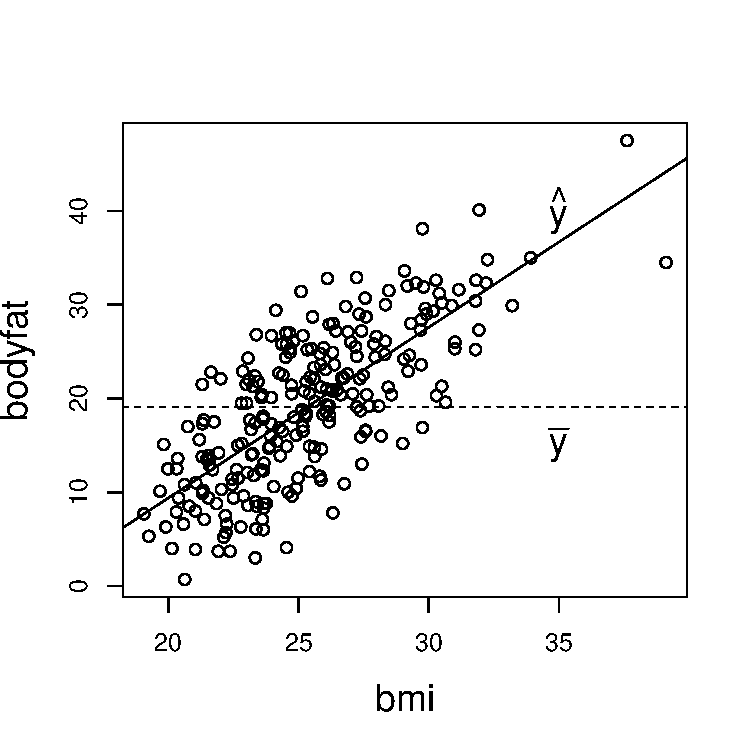
\includegraphics{Bio144_2017_week3-012}
\end{center}
}


\frame[containsverbatim]{
Let us look at the $R^2$s from the two bodyfat models (model 1 with bmi + age, model 2 with bmi + age + neck + hip + abdomen):\\[4mm]

\begin{Schunk}
\begin{Soutput}
[1] 0.5802956
\end{Soutput}
\begin{Soutput}
[1] 0.718497
\end{Soutput}
\end{Schunk}
 ~\\[2mm]
The models thus explain $58$ \% and $72$ \% of the total variability of $y$.\\[5mm]

It thus \emph{seems} that the larger model is ``better''. However, $R^2$ does always increase when new variables are included, but this does not mean that the model is more reasonable. \\[2mm]

\myalert{Model selection} will be a topic that comes later in this course...
}




\frame{\frametitle{Interpretation of the coefficients}
What does the regression output actually \emph{mean}?
}


%\frame{References:
%\bibliographystyle{Chicago}
%\bibliography{refs}
%}

\end{document}
